% Shared standalone design for the editable figure reconstructions.
\documentclass[tikz,border=5pt,10pt]{standalone}
\usepackage[T1]{fontenc}
\usepackage[utf8]{inputenc}
\usepackage{newpxtext,newpxmath}
\usepackage[scaled=.94]{sourcesanspro}
\usepackage{pgfplots}
\pgfplotsset{compat=1.18}
\usetikzlibrary{arrows.meta,calc,positioning,decorations.pathreplacing,
  decorations.markings,patterns,matrix,shapes.geometric,fit,backgrounds,
  intersections,angles,quotes}
\definecolor{ink}{HTML}{203746}
\definecolor{accent}{HTML}{146C78}
\definecolor{muted}{HTML}{667780}
\definecolor{signalred}{HTML}{B94B44}
\color{ink}
\tikzset{>=Latex,line width=.8pt,
  every node/.style={font=\small},
  axis/.style={->,draw=muted,line width=.5pt},
  guide/.style={draw=muted,dashed,line width=.45pt},
  curve/.style={draw=accent,line width=1pt},
  marker/.style={circle,fill=accent,inner sep=1.5pt},
  labelbox/.style={fill=white,inner sep=2pt}}

\begin{document}
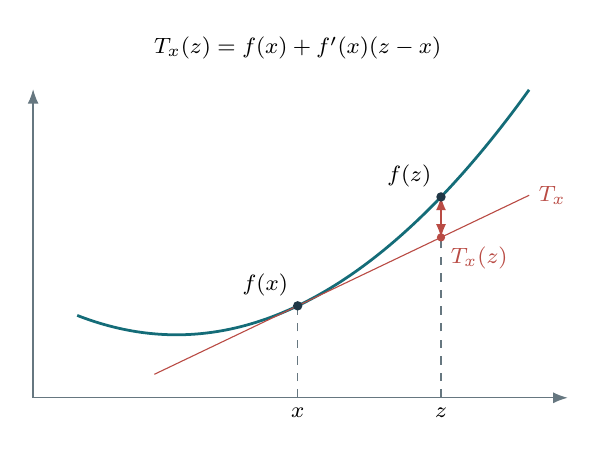
\begin{tikzpicture}[x=0.7cm,y=0.8cm,every node/.style={font=\footnotesize}]

\draw[axis] (0,0)--(9.7,0);\draw[axis] (0,0)--(0,4.9);
\draw[curve] plot[domain=.8:9,samples=101] (\x,{.095*(\x-2.6)^2+1});
\draw[signalred] (2.2,.373)--(9,3.2154) node[right] {$T_x$};
\coordinate (X) at (4.8,1.4598);\coordinate (Z) at (7.4,3.1888);\coordinate (TZ) at (7.4,2.5466);
\draw[guide] (4.8,0)--(X) (7.4,0)--(Z);\draw[signalred,<->] (TZ)--(Z);
\fill[ink] (X) circle (1.7pt) (Z) circle (1.7pt);\fill[signalred] (TZ) circle (1.5pt);
\node[below] at (4.8,0) {$x$};\node[below] at (7.4,0) {$z$};\node[above left] at (Z) {$f(z)$};\node[above left] at (X) {$f(x)$};
\node[below right,signalred] at (TZ) {$T_x(z)$};
\node at (4.8,5.55) {$T_x(z)=f(x)+f'(x)(z-x)$};
\end{tikzpicture}
\end{document}
